%!TEX root = ../main.tex


\begin{titlepage}

% Kensington picture
\begin{tikzpicture}[remember picture,overlay] 
    \node[anchor=north, yshift=-10mm] (jcd_pic) at (current page.north){
        % // ToDo : Remplacer par une photo sans marque de luxe / modèles
        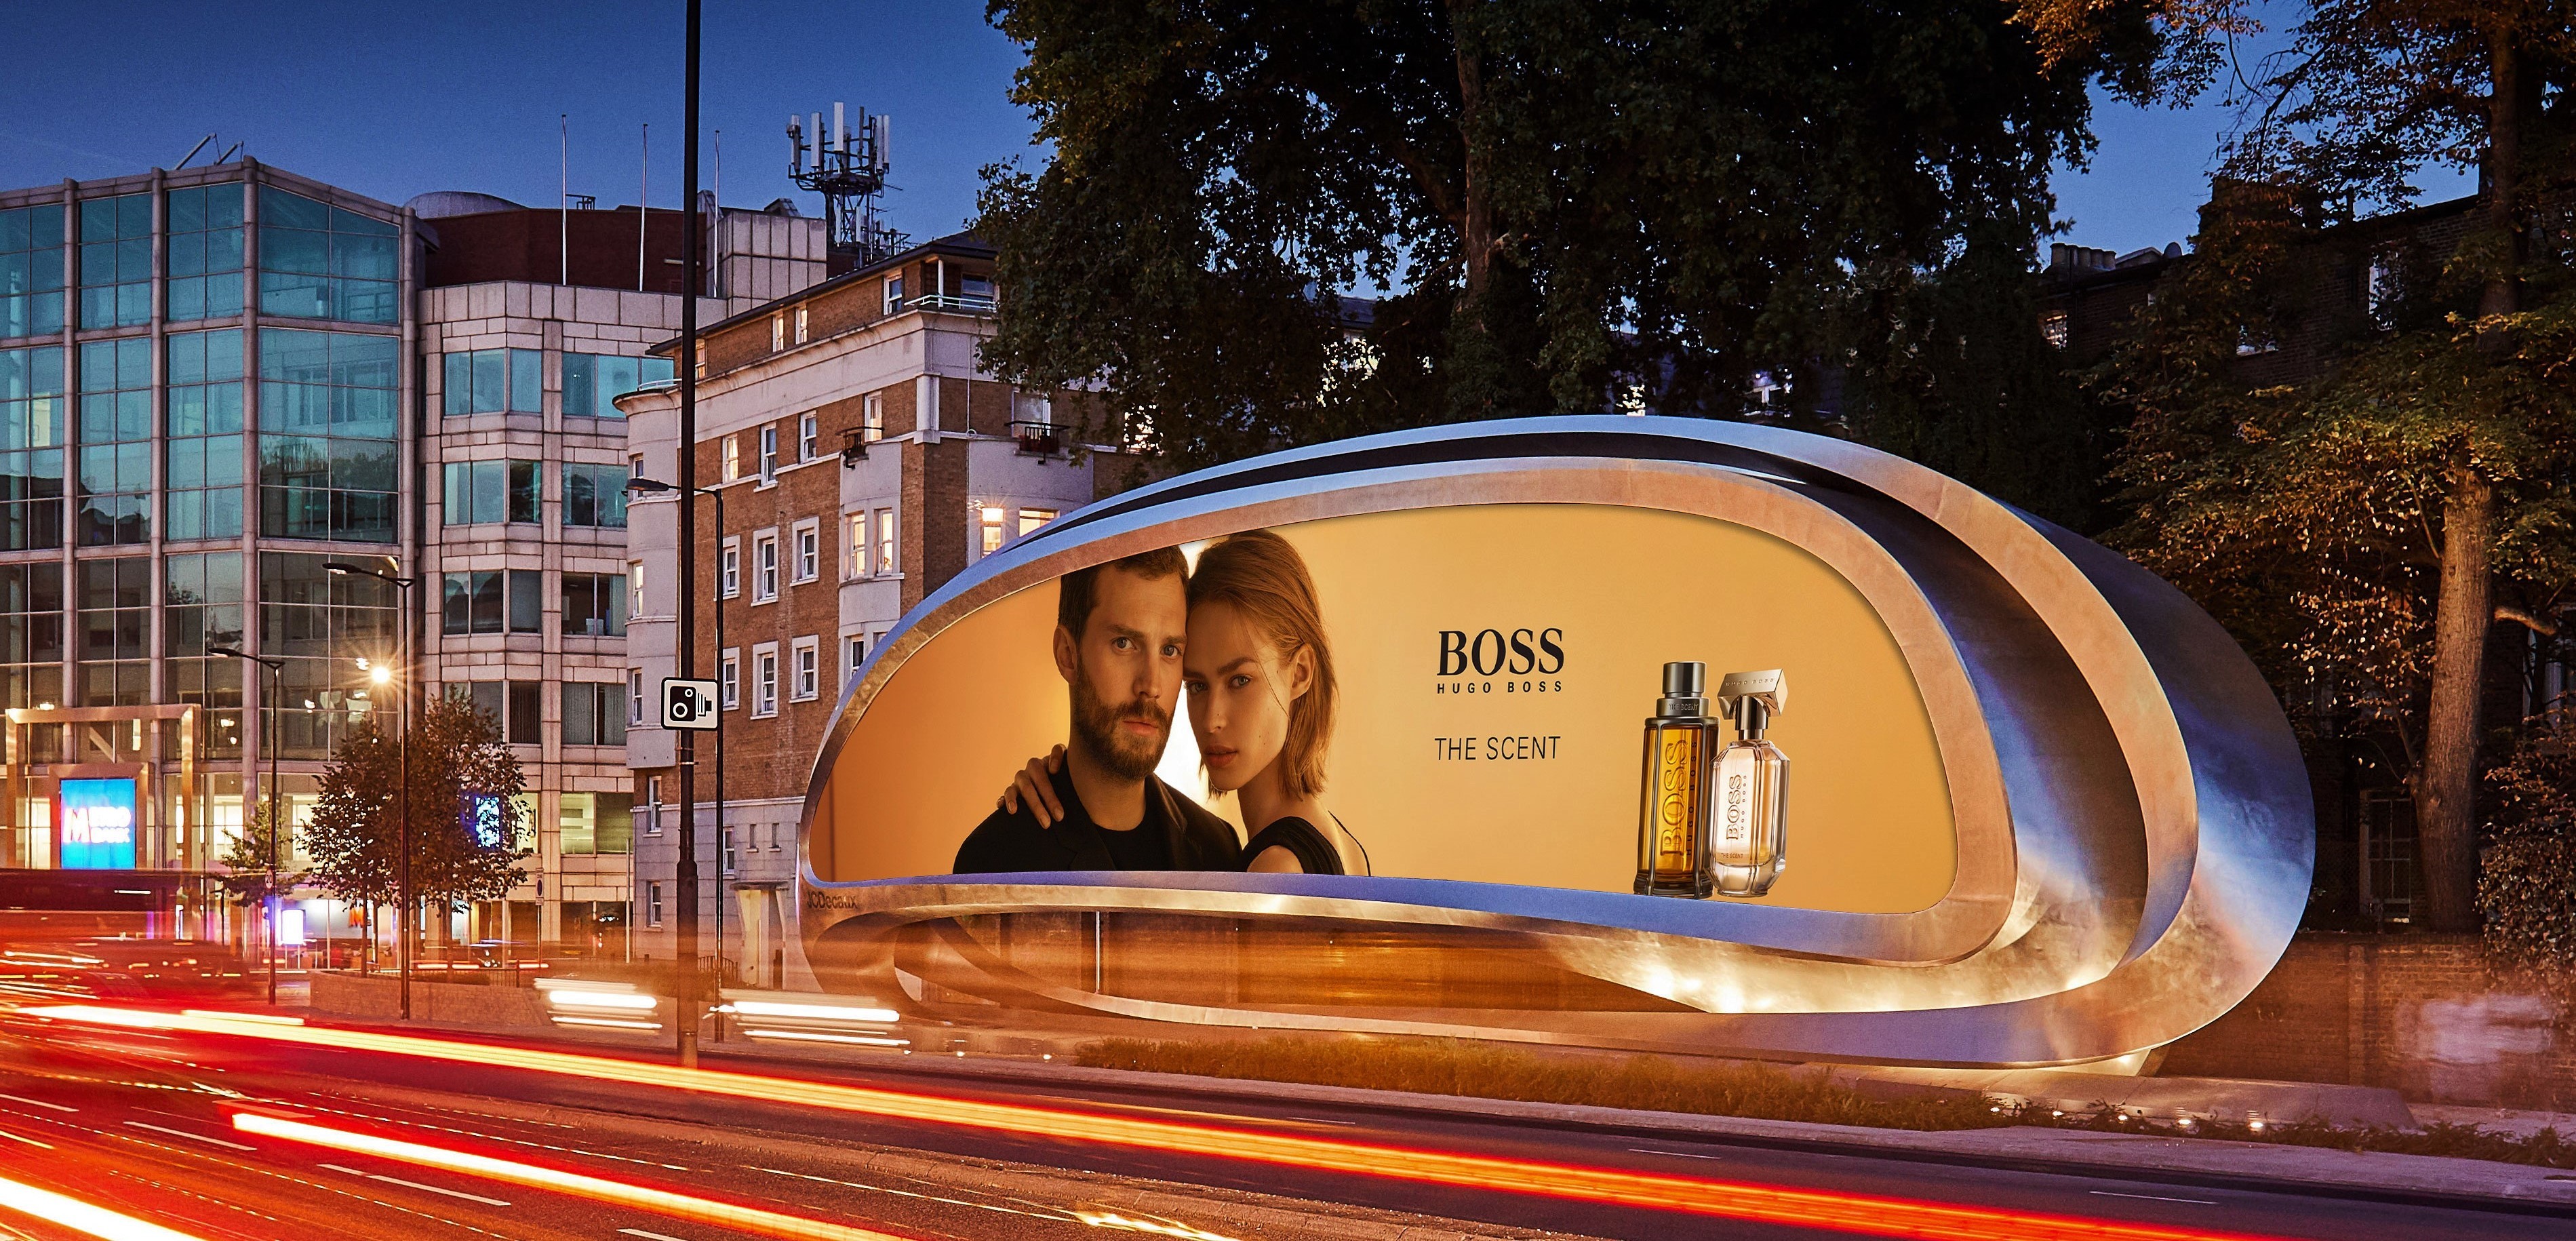
\includegraphics[width=0.9\paperwidth,height=0.45\paperheight]{resources/img/jcd_background.jpg}
    };
\end{tikzpicture}

% Blue box (ugly way make it, but will do the job)
\begin{tikzpicture}[remember picture,overlay] 
    \node[anchor=north, yshift=-0.44\paperheight] at (current page.north){
        
\includegraphics[width=0.9\paperwidth,height=0.145\paperheight]{resources/img/blue_bg.jpg}

    };
    \node[anchor=north, yshift=-0.46\paperheight, xshift=-0.44\paperwidth, align=flush right, text width=0.7\paperwidth] 
    at (current page.north east) {
        \color{white} \Huge \textbf\documenttype\\
        \vspace{5mm}
        \color{white} \LARGE \documenttitle\\
    };
    \node[anchor=north, yshift=-0.64\paperheight, align=center, text width=0.7\paperwidth] at (current page.north) {
        \Large \textbf{Auteur:} Lucas GRELAUD\\
        \vspace{2mm}
        \Large \textbf{Période de mission :} 8 Février 2021 au 26 Août 2021
    };
    \node[anchor=north, yshift=-0.74\paperheight] at (current page.north) {
        \large
        \begin{tabular}{c@{\hskip 20mm}c@{\hskip 20mm}c}
    
            \textbf{\underline{Maître d'apprentissage}} & \textbf{\underline{Président du Jury}} & \textbf{\underline{Tuteur pédagogique}}\\
            \\
            \corpmanager & \jurypresident & \documentreviewer
        \end{tabular}
    };

\end{tikzpicture}

% ESIEA logo
\begin{tikzpicture}[remember picture,overlay] 
    \node[anchor=north, xshift=0.25\paperwidth] at (current page.north west){
        
\includegraphics[width=0.45\paperwidth,keepaspectratio]{resources/img/Logo_ESIEA_Baseline_blanc.png}
    };
\end{tikzpicture}

% Additionnal info
\begin{tikzpicture}[remember picture,overlay] 
    \node[anchor=south, yshift=-0.46\paperheight, xshift=-0.44\paperwidth, align=flush right, text width=0.7\paperwidth] 
    at (current page.south east) {
        \textbf\documenttype\\
        \vspace{5mm}
        \color{white} \LARGE \documenttitle\\
    };

\end{tikzpicture}

% JCDecaux logo
\begin{tikzpicture}[remember picture,overlay] 
    \node[anchor=south, yshift=15mm] at (current page.south){
        
\includegraphics[width=0.25\paperwidth,keepaspectratio]{resources/img/Logo_JCDecaux_seul_without_baseline.jpg}
    };
\end{tikzpicture}

\end{titlepage}

